%
%  NumGenerator
%
%  Created by vbosch on 2011-04-18.
%  Copyright (c) 2011 McBosch. All rights reserved.
%
\documentclass[a4paper,10pt,titlepage]{article}

% Use utf-8 encoding for foreign characters
\usepackage[utf8]{inputenc}

% Setup for fullpage use
\usepackage{fullpage}
\usepackage{titlepic}
\usepackage{float}
\usepackage{color}

% Uncomment some of the following if you use the features
%
% Running Headers and footers
%\usepackage{fancyhdr}

% Multipart figures
%\usepackage{subfigure}

% More symbols
\usepackage{amsmath}
%\usepackage{amssymb}
%\usepackage{latexsym}

% Surround parts of graphics with box
\usepackage{boxedminipage}

% Package for including code in the document
\usepackage{listings}

% If you want to generate a toc for each chapter (use with book)
\usepackage{minitoc}

% This is now the recommended way for checking for PDFLaTeX:
\usepackage{ifpdf}

%\newif\ifpdf
%\ifx\pdfoutput\undefined
%\pdffalse % we are not running PDFLaTeX
%\else
%\pdfoutput=1 % we are running PDFLaTeX
%\pdftrue
%\fi

\ifpdf
\usepackage[pdftex]{graphicx}
\else
\usepackage{graphicx}
\fi
\title{RES \\ Course Work - Part 1 Exercises}
\titlepic{
\includegraphics[width=250pt]{cover.jpg}}
\author{Vicente Bosch Campos \dag \\
\textcolor{blue}{\texttt{viboscam@posgrado.upv.es}}}

\begin{document}

\ifpdf
\DeclareGraphicsExtensions{.pdf, .jpg, .tif}
\else
\DeclareGraphicsExtensions{.eps, .jpg}
\fi

\maketitle

\tableofcontents

\listoffigures

\newpage

\section{Introduction}
\subsection{Context}

\par For the RES part 1 course work proposed by Daniel Keysers we will perform the following exercises:
\begin{itemize}
	\item 1.3 Implementation of the three binarization methods discussed in class: Simple iteration of means, Otsu's and Niblack's.
	\item 1.4 Write a program that given an image it computes all connected regions and represents the results as an image.
\end{itemize}

\subsection{Scope}

\par In order to implement and evaluate the techniques we will develop code in order to cover the following user cases:
\begin{itemize}
	\item Launching a command to binarize an image where the user is able to indicate: input image, output image, save result to file or just show in screen, binarization algorithm and algorithm input parameters.
	\item Launching a command to binarize an image, detect the connected regions and display a result to the user. The user must be able to indicate: input image, out image, binarization algorithm, algorithm input parameters, neighbourhood function to review for each pixel ( 4 or 8).
\end{itemize}

\section{Development}
\par For our implementation of the exercises we have implemented the algorithms in Ruby (v1.9.2) and the following libraries where used: 
\begin{description}
	\item[RMagick (2.13.1):] RMagick is a wrapper library for the Image Magick software. RMagick has been used in our implementation to load, draw on and save images. 
	\item[Trollop (1.16.2):] Trollop was used in order to parse and generate validators of the command line options for the image\_binarization and connected\_components commands created.  
	\item[Awesome Print (0.3.1):] Used to perform pre-formatted human readable print outs of the objects.
\end{description}

\subsection{Program Structure}

\par Next we will detail the main software components and characteristics for the exercise resolution. The implementation can be divided in the following main software components:
\begin{description}
	\item[Image binarization command:] Present in \textit{./bin/image\_binarization.rb}. This file is in charge of parsing the  command line options (with the use of the library trollop) and instantiating the objects according to the user input for the image binarization exercise. Main purpose of this component is to facilitate execution and separate the library implementation from the commands generated. 
	\item[Connected components command:]  Can be found in \textit{./bin/connected\_components.rb}. This file is in charge of parsing the  command line options (with the use of the library trollop) and instantiating the objects according to the user input for the connected components exercise. Main purpose of this component is to facilitate execution and separate the library implementation from the commands generated. 
	\item[Image class:] Coded in \textit{./lib/image.rb}. The image class is the main class of both exercise implementations as we are performing operations on images. The class provides the following methods:
	\begin{itemize}
		\item initialize - Is called upon object creation. The initialize methods performs the following actions:
		\begin{itemize}
			\item Loads the image with the help of the RMagick library
			\item Extracts the image grey scale by copying the intensity channel.
			\item Calculates the standard integral image and the sum of squares integral image.
			\item Calculates the normalized histogram from the intensity matrix
		\end{itemize}
		\item image\_rows - returns the number of pixel rows in the image.
		\item image\_columns - return the number of pixel columns in the image.
		\item obtain\_image\_intensity\_matrix - helper method used to obtain the array of pixels of the image with just the intensity channel information and then load it into a Matrix object with the help of the Array slice method. 
		\item calculate\_integral\_images - calculates the integral images by iterating through the intensity matrix (either stored on the object or passed through parameters) as per the usual integral images calculation algorithms. It stores the results into some object variables for further use.
		\item mean\_of\_region - given a point x,y of the image and a region height and width it returns the mean value of the intensity matrix for that region. The method implements the standard algorithm to return the mean with the use of the integral image but also checks for border conditions so that if the region provided exceeds the borders of the matrix then the mean is returned of the region that is inside. If no region is provided then the mean of the whole image is given. 
		\item standard\_deviation\_of\_region - same as for the mean\_of\_region method but in this case it uses the sum of squares integral image to calculate the variance and from this return the positive square root to calculate the deviation. 
		\item intensity\_matrix\_to\_image - given an intensity matrix it generates a new image object by loading the elements of the matrix as an array to the image constitute method.
		\item to\_file - saves an image to an specific file path.
		\item apply\_threshold - iterates through the whole image applying a set threshold to binarize the image and returns a new intensity matrix. 
		\item simple\_binarization - performs the simple means binarization algorithm. Iterations are performed until there is a difference lower than 0.0001 between the old and new threshold.
		\item otsu\_binarization - performs Otsu's binarization algorithm for a given intensity matrix. Total sum of the histogram is performed inside this method. Since our histogram is represented as a hash and we can iterate through the buckets with values we do not have to perform checks inside the loop regarding empty/non-empty bucket. 
		\item niblack\_binarization - implementation of Niblack's binarization algorithm for a given intensity matrix. The method performs a processing for each pixel in the image by selecting the below corner of the image that contains the current pixel being processed. 
		\item binarize! - performs the binarization algorithm on the current image modifying its internal representation. 
		\item draw\_intensity\_matrix - displays the image represented in the intensity matrix.
		\item draw\_binary\_image - performs binarization algorithm on the image and shows the result on the screen but does not modify the internal representation, hence the image object remains untouched. 
		\item save\_binary\_image performs binarization algorithm on the image and saves the result to a file but does not modify the internal representation, hence the image object remains untouched.
		\item detect\_connected\_regions - performs the connected region algorithm on the image. Our implementation performs the following changes on the standard implementation:
		\begin{itemize}
			\item As per our image format the black pixels are represented with 0 hence we will not evaluate the pixels with value one.
			\item We store in a matrix the region label assigned to each pixel, being 0 the label of no region assigned.
			\item We store in a hash the translation between regions. Hence if the region has not been absorbed by another they key in the hash will be equal to the value.
			\item If a region is absorbed by another the region label of least number will absorb the rest. In this manner we can afterwards guarantee that the class equivalence can be computed linearly.
			\item We present the result to the user by displaying the image drawing in different color sets each of the connected regions.
		\end{itemize}
		\item neighbour\_labels\_set - returns an ordered set of the labels of the adjacent pixels as per the type of neighbourhood selected ( 4 or 8 ). As we use an ordered set this guarantees we do not duplicate labels and that in the first position we have the label of least value. 
		\item extract\_regions - extracts the list of pixels assigned to each of the regions for its drawing. 
		\item draw\_connected\_regions - draws each of the regions on top of the original image. It assigns the region a color by performing a round robin over a predefined set of colors. 
	\end{itemize}
	\item[Matrix extension class:] It is an extension performed by us over the standard matrix class, can be found in in \textit{./lib/extendmatrix2.rb} to perform fast calculation over the matrix without replicating objects and also to add the new histogram methods.
	\item[Application logger:] Utility class coded in in \textit{./lib/application\_logger.rb} to provide the application with a unique standard logger object by using the singleton pattern. 
\end{description}	
		
\subsection{Command Options}

\subsubsection{Image binarization command}

\par The command \textit{image\_binarization.rb} allows several execution options that can be listed when executing  \textit{image\_binarization.rb -h} which we will now describe in detail:
\begin{description}
	\item[Mode (-m):] Indicates in what mode must the binarization command be launched. Screen just shows the result on the current computers display and file saves the result to an image. Default mode is screen.
	\item[Input image (-i):] File path to the image to binarize.
	\item[Output image (-o):] Only used if the command is executed in file mode. This parameter indicates where to save the resulting image, the format indicated in the name will be used as format to save the image. Default output file is ./output.png.
	\item[Algorithm (-a):] Binarization algorithm to apply to the image: simple, otsu, niblack. By default the algorithm used will be simple. 
	\item[Niblack region size (-n):] height and width to be considered around each pixel when being processed in order to get the mean and standard deviation. By default the values are set to 15 15.
	\item[Version (-v):] Prints out the current version of the program.
	\item[Help (-h):] Prints outs the help text with the options explained above.

\end{description}

\subsubsection{Connected components command}

\par The command \textit{connected\_components.rb} allows several execution options that can be listed when executing  \textit{connected\_components.rb -h} which we will now describe in detail:
\begin{description}
	\item[Input image (-i):] File path to the image to binarize and detect connected regions. 
	\item[Output image (-o):] This parameter indicates where to save the resulting image, the format indicated in the name will be used as format to save the image. Default output file is ./output.png.
	\item[Neighbourhood (-n):] Determines the type of neighbourhood to consider when studying the adjacent pixels in order to detect continuous regions. By default it is set to 4.  
	\item[Algorithm (-a):] Binarization algorithm to apply to the image: simple, otsu, niblack. By default the algorithm used will be simple. 
	\item[Niblack region size (-b):] height and width to be considered around each pixel when being processed in order to get the mean and standard deviation. By default the values are set to 15 15.
	\item[Version (-v):] Prints out the current version of the program.
	\item[Help (-h):] Prints outs the help text with the options explained above.

\end{description}

\subsection{Command Outputs}

\subsubsection{Image Binarization}

\par The generated code will present us with the following outputs:
\begin{description}
	\item[Screen mode:] In this case the program will output the following messages:
		{\footnotesize\begin{verbatim}
		veraw76-30:bin vbosch$ ./image_binarization.rb -i ../test/bridge.jpg -a niblack -n 51 51
		I, [2011-05-11T09:44:49.061250 #29275]  INFO -- : Loading image
		I, [2011-05-11T09:44:49.290104 #29275]  INFO -- : Calculating integral images
		I, [2011-05-11T09:44:54.306320 #29275]  INFO -- : Calculating normalized intensitiy histogram
		I, [2011-05-11T09:44:54.881402 #29275]  INFO -- : Performing niblack_binarization binarization on image
		I, [2011-05-11T09:45:10.592145 #29275]  INFO -- : Drawing intensity matrix
		I, [2011-05-11T09:45:10.592255 #29275]  INFO -- : Transforiming intensity matrix to image
		\end{verbatim}}
	\item[File mode:] For the other case the program will present the messages:
	{\footnotesize\begin{verbatim}
		veraw76-30:bin vbosch$ ./image_binarization.rb -m file -i ../test/bridge.jpg -a niblack -n 51 51
		I, [2011-05-11T09:45:47.777583 #29283]  INFO -- : Loading image
		I, [2011-05-11T09:45:47.906483 #29283]  INFO -- : Calculating integral images
		I, [2011-05-11T09:45:52.996463 #29283]  INFO -- : Calculating normalized intensitiy histogram
		I, [2011-05-11T09:45:53.575912 #29283]  INFO -- : Performing niblack_binarization binarization on image
		I, [2011-05-11T09:46:09.394624 #29283]  INFO -- : Transforiming intensity matrix to image
		I, [2011-05-11T09:46:09.458272 #29283]  INFO -- : Saving image to path: ./output.png
	\end{verbatim}}
\end{description}

\subsubsection{Connected Components}

\par The generated code will present us with the following output:
{\footnotesize\begin{verbatim}

veraw76-30:bin vbosch$ ./connected_components.rb -i ../test/bridge.jpg -a niblack -n 8 -b 15 15
I, [2011-05-11T09:48:10.901261 #29294]  INFO -- : Loading image
I, [2011-05-11T09:48:11.030034 #29294]  INFO -- : Calculating integral images
I, [2011-05-11T09:48:16.018455 #29294]  INFO -- : Calculating normalized intensitiy histogram
I, [2011-05-11T09:48:16.605310 #29294]  INFO -- : Performing niblack_binarization binarization on image
I, [2011-05-11T09:48:34.225389 #29294]  INFO -- : IMAGE CHANGED!! Recalculating internal representation
I, [2011-05-11T09:48:34.225613 #29294]  INFO -- : Transforiming intensity matrix to image
I, [2011-05-11T09:48:34.325461 #29294]  INFO -- : Calculating integral images
I, [2011-05-11T09:48:42.525411 #29294]  INFO -- : Detecting connected regions
I, [2011-05-11T09:49:02.590800 #29294]  INFO -- : Translating region labels as per equivalence detected
I, [2011-05-11T09:49:02.594989 #29294]  INFO -- : Extracting regions to drawable format
I, [2011-05-11T09:49:02.991374 #29294]  INFO -- : Drawing regions
I, [2011-05-11T09:49:15.846910 #29294]  INFO -- : Saving image to path: ./output.png

\end{verbatim}}

\section{Experimental Results}

\par Next we will perform some minor tests for each of the commands and present the results for evaluation.

\subsubsection{Image Binarization}

\par For the image binarization command the test image has been of an old aqueduct:

\par \begin{figure}[H]
	\centerline{%
	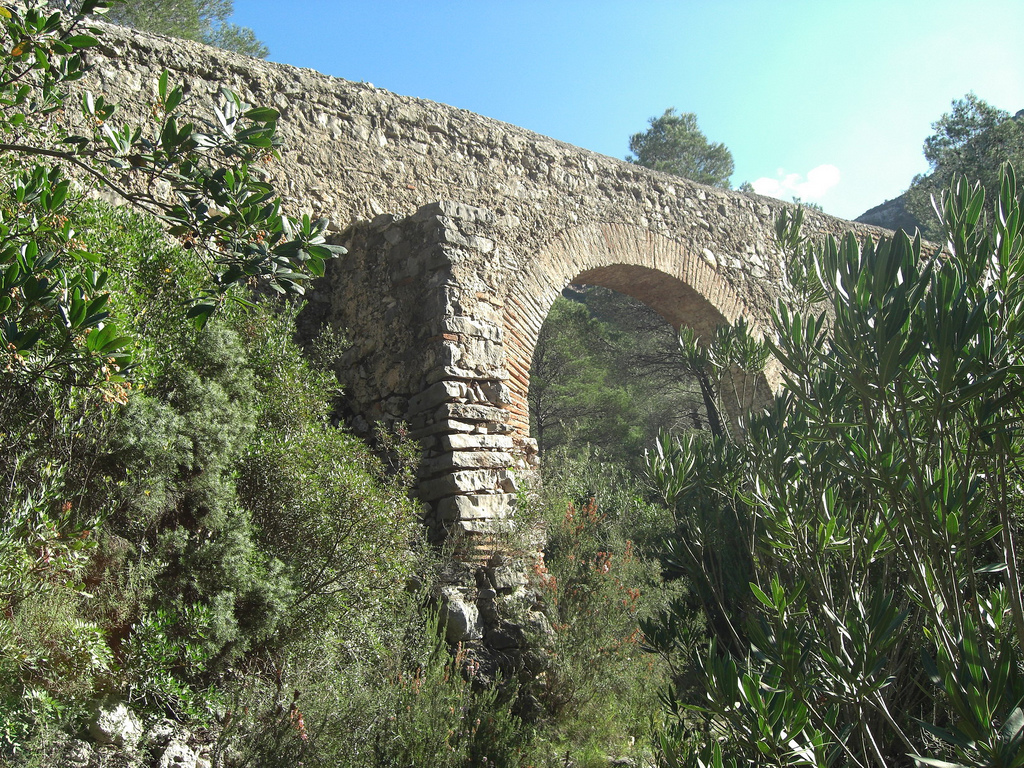
\includegraphics[scale=0.3]{./images/bridge.jpg}
	}
	\caption[Original base aqueduct image]{Image shows the sample test image used for the binarization command review. The image is of an old aqueduct in the mountains near the town of Simat de la Valldigna}
\end{figure}

\par The output when applying the simple binarization algorithm
{\footnotesize\begin{verbatim}
./image_binarization.rb -m file -i ../test/bridge.jpg -o simple.png -a simple
\end{verbatim}}

\par \begin{figure}[H]
	\centerline{%
	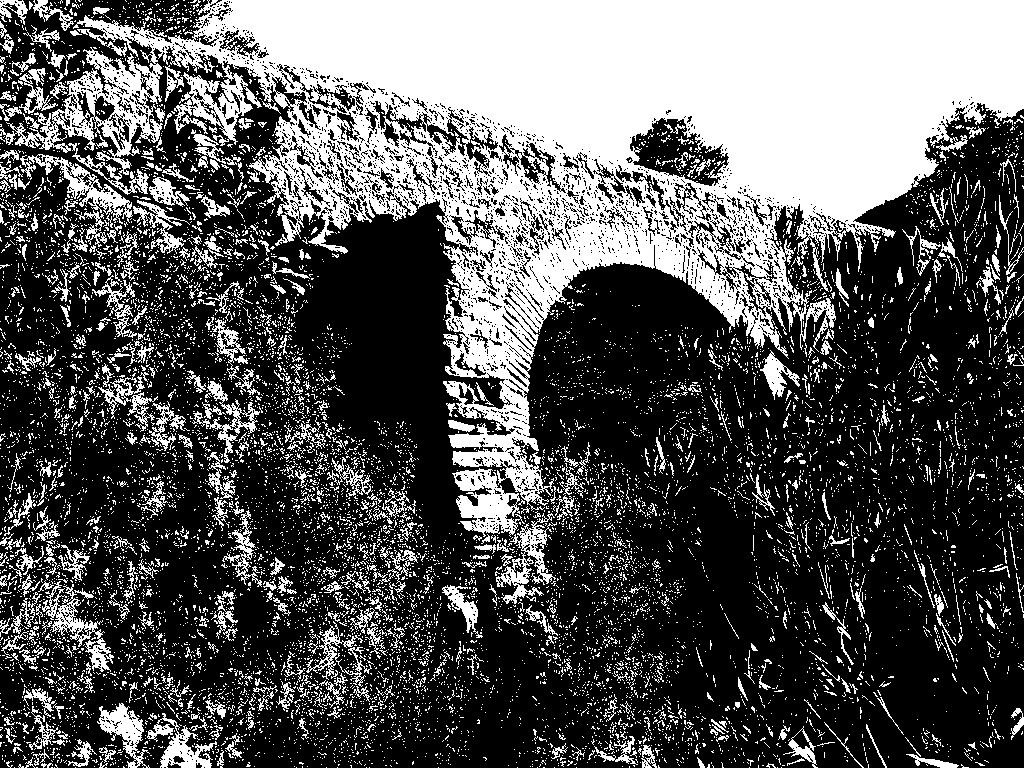
\includegraphics[scale=0.3]{./images/simple.png}
	}
	\caption[Simple binarization sample]{Image shows the result image when we apply the simple binarization algorithm on the aqueduct test.}
\end{figure}


\par The output when applying the Otsu's binarization algorithm
{\footnotesize\begin{verbatim}
./image_binarization.rb -m file -i ../test/bridge.jpg -o otsu.png -a otsu
\end{verbatim}}

\par \begin{figure}[H]
	\centerline{%
	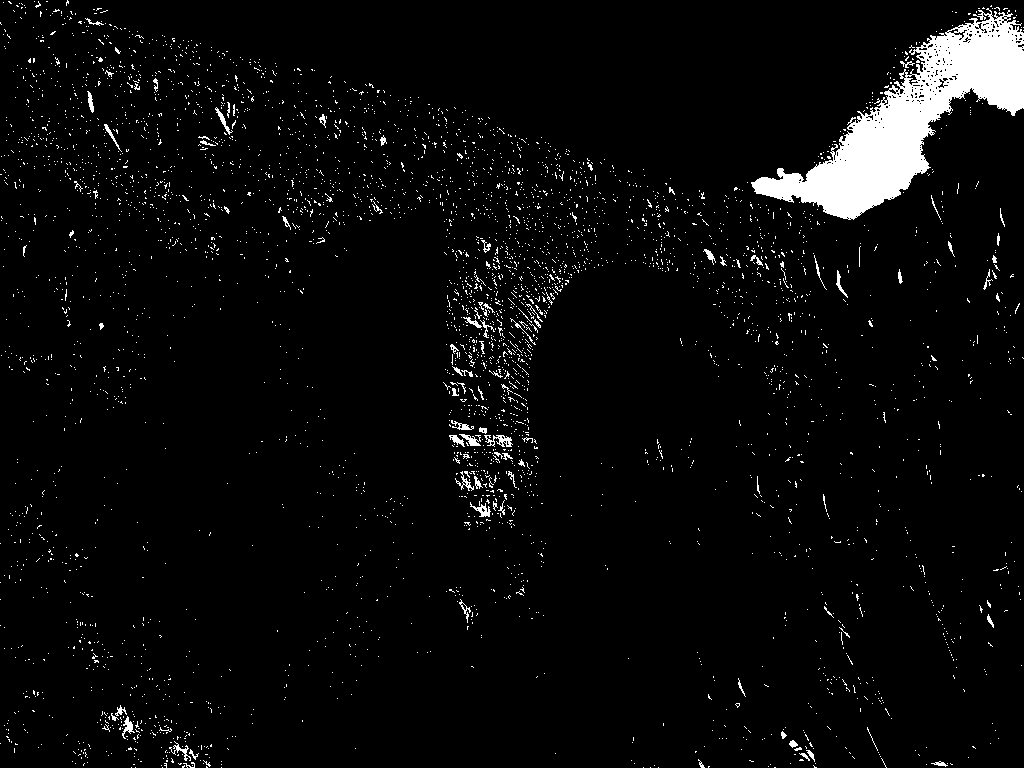
\includegraphics[scale=0.3]{./images/otsu.png}
	}
	\caption[Otsu's binarization sample]{Image shows the result image when we apply Otsu's binarization algorithm on the aqueduct 
test.}
\end{figure}

\par The output when applying the Niblack's binarization algorithm
{\footnotesize\begin{verbatim}
./image_binarization.rb -m file -i ../test/bridge.jpg -o niblack_15_15.png -a niblack -n 15 15
\end{verbatim}}	

\par \begin{figure}[H]
	\centerline{%
	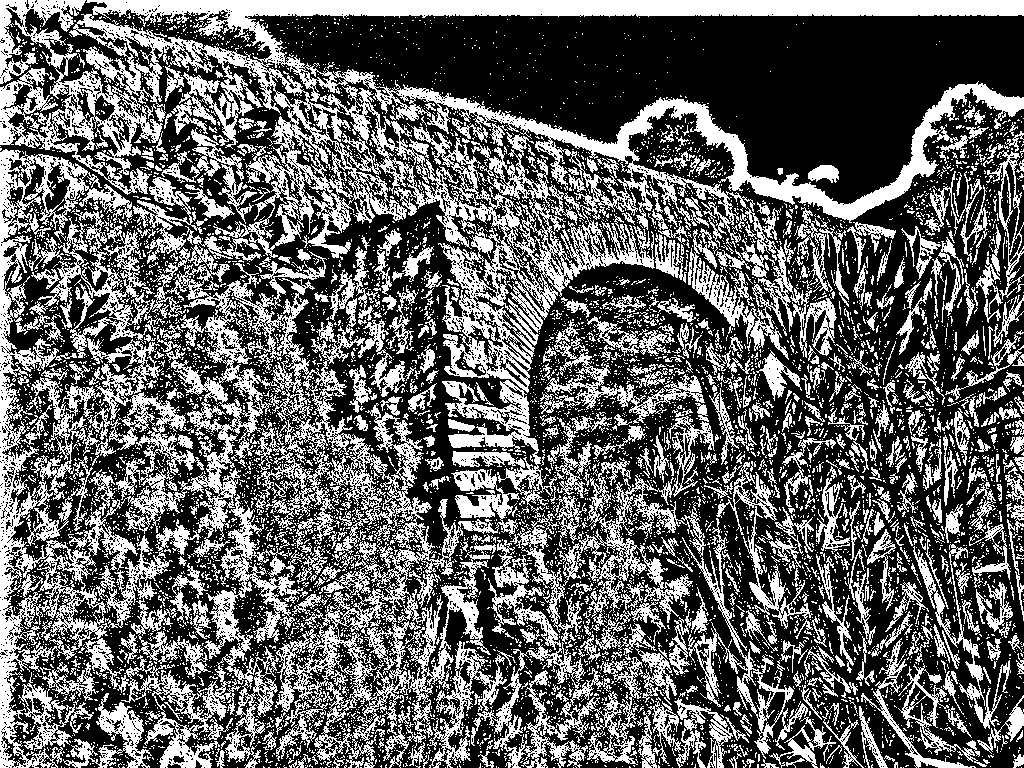
\includegraphics[scale=0.3]{./images/niblack_15_15.png}
	}
	\caption[Niblack's binarization sample 15 x 15 ]{Image shows the result image when we apply Niblack's binarization algorithm on the aqueduct test with a region of 15 x 15}
\end{figure}

{\footnotesize\begin{verbatim}
./image_binarization.rb -m file -i ../test/bridge.jpg -o niblack_51_51.png -a niblack -n 51 51
\end{verbatim}}

\par \begin{figure}[H]
	\centerline{%
	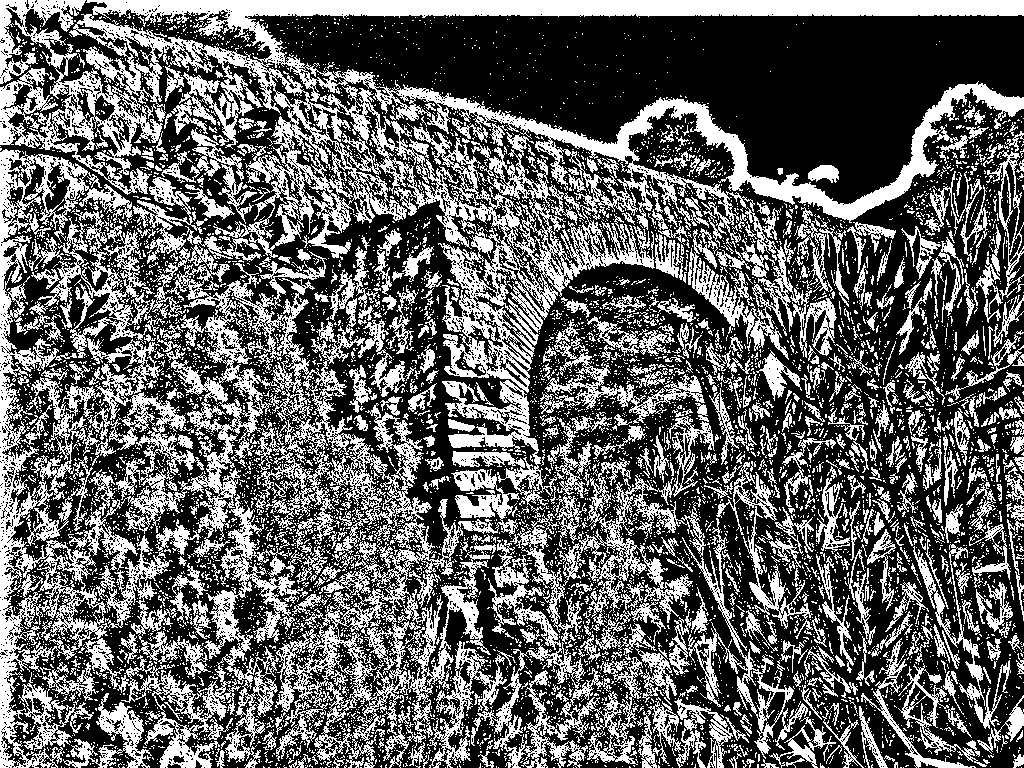
\includegraphics[scale=0.3]{./images/niblack_51_51.png}
	}
	\caption[Niblack's binarization sample 51 x 51 ]{Image shows the result image when we apply Niblack's binarization algorithm on the aqueduct test with a region of 51 x 51}
\end{figure}

{\footnotesize\begin{verbatim}
./image_binarization.rb -m file -i ../test/bridge.jpg -o niblack_201_201.png -a niblack -n 201 201
\end{verbatim}}

\par \begin{figure}[H]
	\centerline{%
	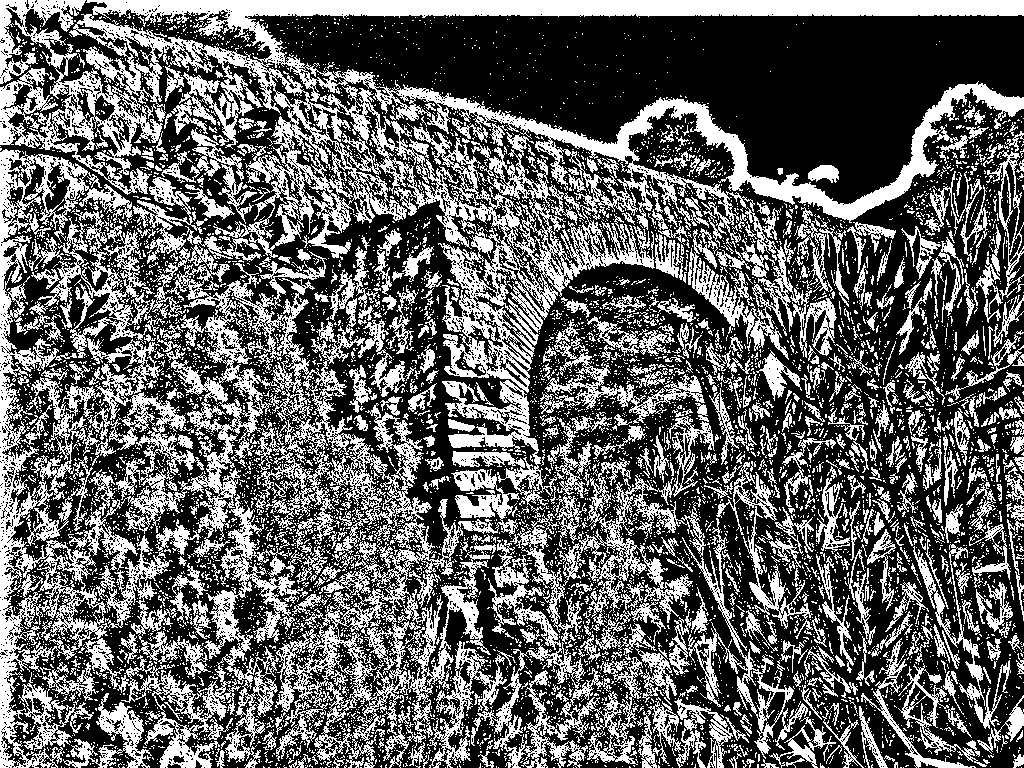
\includegraphics[scale=0.3]{./images/niblack_201_201.png}
	}
	\caption[Niblack's binarization sample 201 x 201 ]{Image shows the result image when we apply Niblack's binarization algorithm on the aqueduct test with a region of 201 x 201}
\end{figure}
	
\subsubsection{Connected Components}

\par For the connected components command the test image has been of a barcode:

\par \begin{figure}[H]
	\centerline{%
	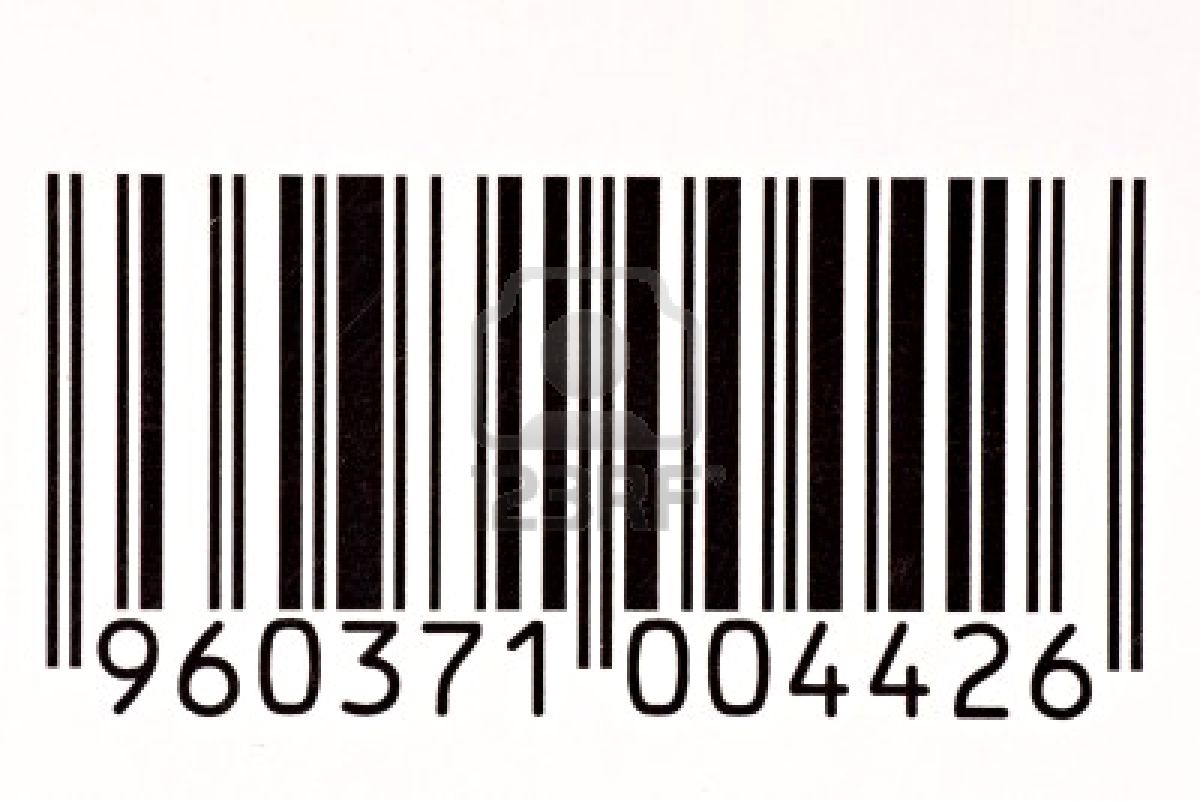
\includegraphics[scale=0.3]{./images/barcode.jpg}
	}
	\caption[Original barcode image]{Image shows the sample test image used for the connected components command review. The image is of sample barcode obtained from the web}
\end{figure}

\par The output when applying the connected regions algorithm prior binarization with the simple algorithm. 
{\footnotesize\begin{verbatim}
./connected_components.rb -i ../test/barcode.jpg -a simple -n 8 -o barcode_simple.png
\end{verbatim}}
\par \begin{figure}[H]
	\centerline{%
	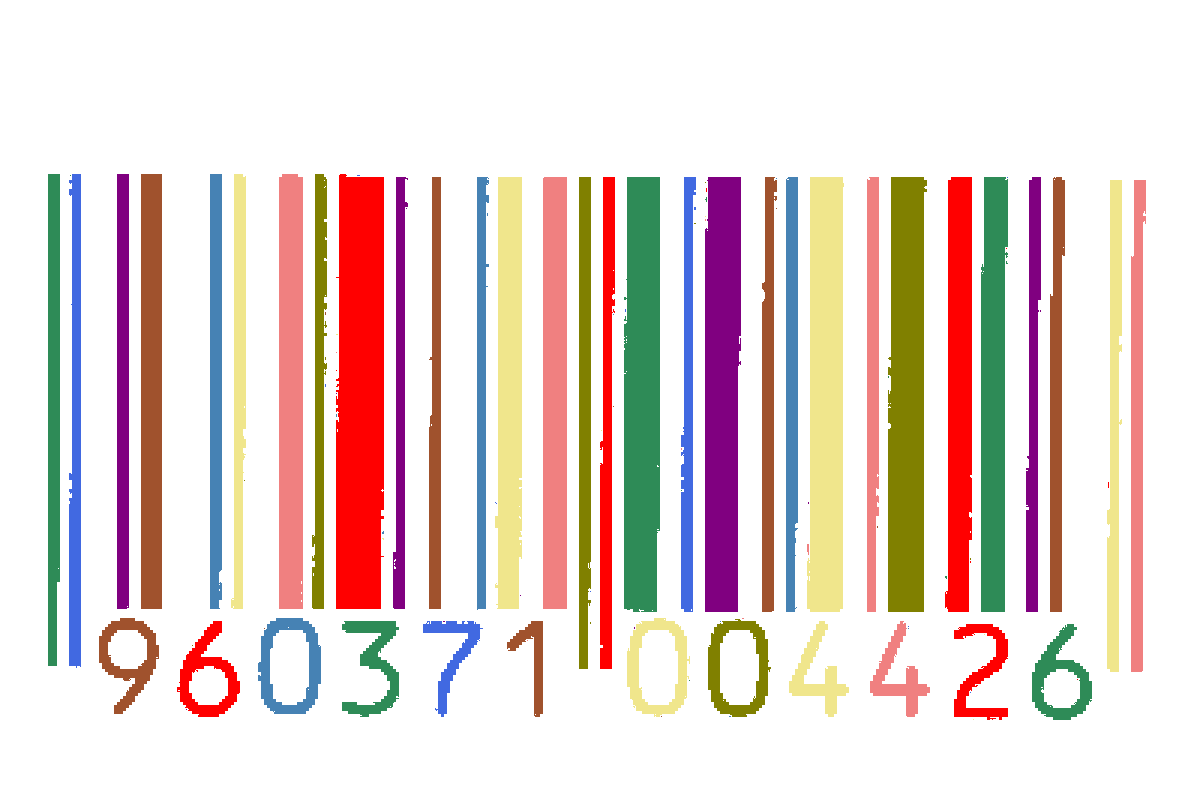
\includegraphics[scale=0.3]{./images/barcode_simple.png}
	}
	\caption[Connected regions execution barcode image]{Image shows the result of executing the connected regions algorithm with 8 neighbours on the test barcode image.}
\end{figure}


\end{document}
